\documentclass{article}
\usepackage[legalpaper, margin=0.5in]{geometry}

\usepackage[utf8]{inputenc} % allow utf-8 input
\usepackage[T1]{fontenc}    % use 8-bit T1 fonts
\usepackage{hyperref}       % hyperlinks
\usepackage{url}            % simple URL typesetting
\usepackage{booktabs}       % professional-quality tables
\usepackage{amsfonts}       % blackboard math symbols
\usepackage{nicefrac}       % compact symbols for 1/2, etc.
\usepackage{microtype}      % microtypography

\usepackage{amsmath}
\usepackage{amssymb}
\usepackage{dsfont}

\usepackage{graphicx}  %Required

\usepackage[font=small,labelfont=sf,skip=0pt]{caption}
\usepackage[caption=true,font=small,labelfont=sf,textfont=sf,skip=0pt]{subfig}
\usepackage{wrapfig}
\usepackage{floatrow}

\DeclareMathOperator*{\argmin}{arg\,min}
\DeclareMathOperator*{\argmax}{arg\,max}

\title{GLAD: {\bf GL}ocalized {\bf A}nomaly {\bf D}etection via Active Feature Space Suppression}

\begin{document}

\maketitle

\section{Introduction}

\begin{figure*}[t]
	\centering
	\captionsetup{labelformat=empty}
	\subfloat{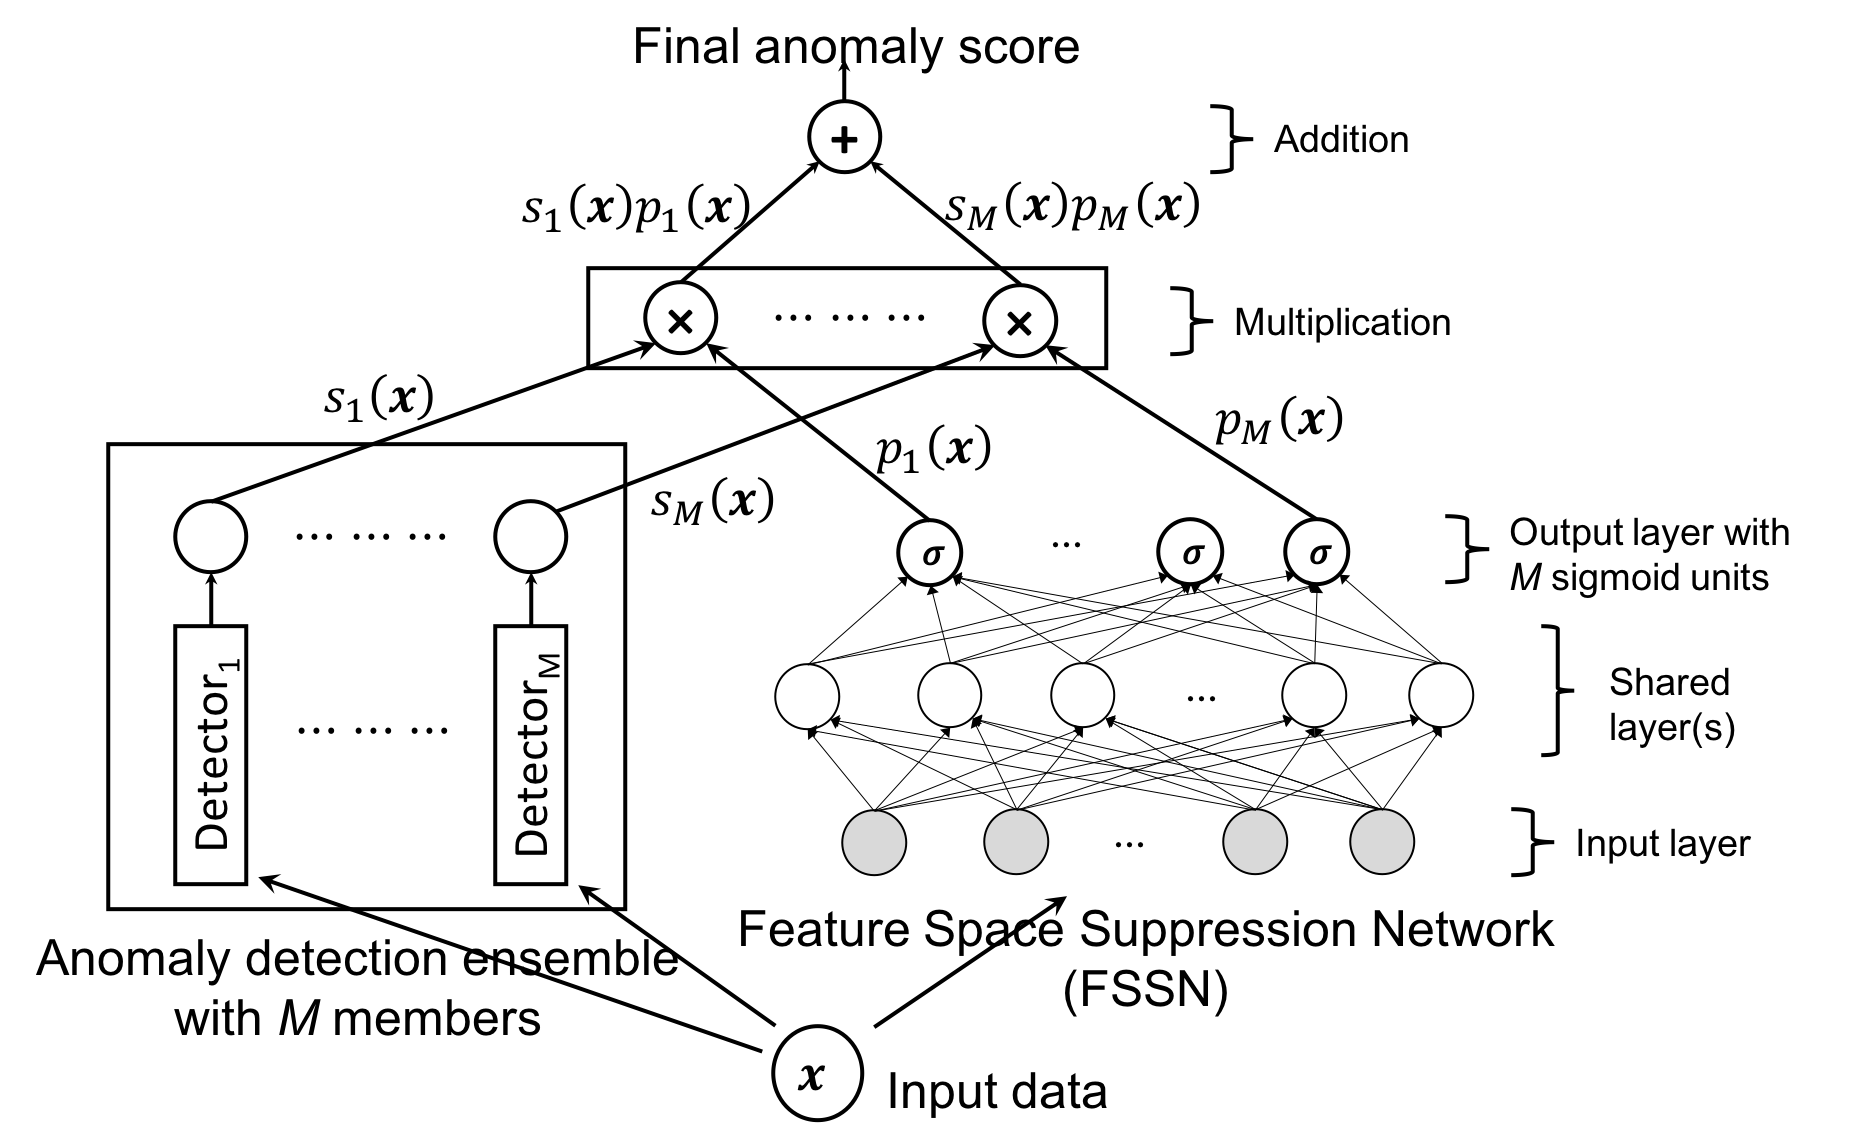
\includegraphics[width=1.0\textwidth]{figures/AFSS.png}} \\[-1ex]
	\caption{GLAD Architecture. The anomaly detection ensemble contains $M$ detectors. We assume that these are all pre-trained and cannot be modified. The final layer of the Feature Space Suppression Network (FSSN) contains $M$ sigmoid outputs, with each one paired with a corresponding ensemble member. Each output node in the FSSN is initially primed to predict the same probability ($0.5$ in our experiments) across the entire feature space. It then receives feedback from the analyst and learns which parts of the feature space are \textit{\textbf{relevant}} for each detector. For an instance ${\bf x}$, $s_m({\bf x})$ denotes the score assigned to it by the $m$-th detector, while $p_m({\bf x})$ denotes the probability computed by the FSSN that the $m$-th detector is relevant. The final anomaly score for an instance ${\bf x}$ is the sum of all its scores from each detector weighted by the corresponding relevances.}
	\label{fig:architecture}
\end{figure*}

\paragraph{Approach} We denote the input space by $\mathcal{X} \subseteq \mathbb{R}^d$. Each instance ${\bf x} \in \mathcal{X}$ is associated with a hidden label $y_i \in \{-1, +1\}$. Instances labeled $+1$ represent the \textit{anomaly} class and are at most a small fraction $\tau$ of all instances. The label $-1$ represents the \textit{nominal} class. We assume that we have an ensemble $\mathcal{E} = \{\mathcal{A}_1, ..., \mathcal{A}_M\}$ of $M$ pre-trained anomaly detectors. In order to customize an anomaly detector $\mathcal{A}_m$ for a particular task, we start by decomposing the anomaly score it assigns to an instance ${\bf x} \in \mathcal{X}$ into two parts: {\bf (a)} the original score $s_m({\bf x})$, and {\bf (b)} the \textit{relevance} $p_m({\bf x}) \in [0, 1]$. The score assigned by $\mathcal{A}_m$ is then $s_m({\bf x})p_m({\bf x})$. The overall anomaly score is computed as: \texttt{Score}$({\bf x}) = \sum_{m=1}^M{s_m({\bf x})p_m({\bf x})}$.

We start with the assumption that each ensemble member is uniformly relevant in every part of the input feature space, i.e., $p_1({\bf x}) = ... = p_M({\bf x}) = const \ \forall {\bf x} \in \mathcal{X}$. This assumption is implemented by priming a neural network referred to as \textit{FSSN} to predict the same probability value $b \in (0, 1)$ for every input (labeled and unlabeled) using the $\ell_{prior}$ loss in Equation~\ref{eqn:prior}. In effect, this places \textit{\textbf{a uniform prior for the relevance of each detector over the input space $\mathcal{X}$}}  (rather than the {\em parameter} space). When all detectors have the same relevance, the final anomaly score simply corresponds to the average score across all detectors (up to a multiplicative constant). This is \textbf{a good starting point for active learning.} Next, the algorithm receives label feedback from an analyst and determines whether the ensemble made an error (i.e., ranked a labeled nominal in the top $\tau$ fraction of instances which are assumed to be anomalous, or ranked a labeled anomaly lower than the top $\tau$ fraction of instances). If so, the FSSN tries to suppress all erroneous detectors for similar inputs using a combination of $\ell_{prior}$ and the AAD loss $\ell_{AAD}$ (Equation~\ref{eqn:l_fssn}).

\begin{align}
\ell_{prior}({\bf x}) &= \sum_{m=1}^M{-b\log(p_m({\bf x})) -(1 - b)\log(1 - p_m({\bf x}))} \label{eqn:prior} \\
\ell_A(q; ({\bf x}_i, y_i)) &= \left \{ 
\begin{array}{lr}
0 & \text{\texttt{Score}$({\bf x}_i)$} \ge q \text{ and $y_i=+1$} \\
0 & \text{\texttt{Score}$({\bf x}_i)$} < q \text{ and $y_i=-1$} \\
(q - \text{\texttt{Score}$({\bf x}_i)$}) & \text{\texttt{Score}$({\bf x}_i)$} < q \text{ and  $y_i=+1$} \\
(\text{\texttt{Score}$({\bf x}_i)$} - q) & \text{\texttt{Score}$({\bf x}_i)$} \ge q \text{ and $y_i=-1$}
\end{array} 
\right. \label{eqn:loss_x_loss} \\
\ell_{AAD} &= \frac{1}{|{\bf H}_f|} \sum_{{\bf x}_i \in {\bf H}_f} \left( \ell_A(\hat{q}_{\tau}^{(t-1)}; ({\bf x}_i, y_i)) + \ell_A(\text{\texttt{Score}}({\bf x}_{\tau}^{(t-1)}); ({\bf x}_i, y_i)) \right) \label{eqn:aad_loss} \\
\ell_{FSSN}({\bf x}) &= \ell_{AAD}({\bf x}) + \lambda \ell_{prior}({\bf x}) \label{eqn:l_fssn} \\
& \text{where $\lambda=1$ works well} \nonumber
\end{align}

$\mathbf{H}_f$ in Equation~\ref{eqn:aad_loss} denotes the set of instances labeled by the analyst. ${\mathbf x}_{\tau}^{(t-1)}$ and $\hat{q}_{\tau}^{(t-1)}$ are the instance and the score resp. ranked at the $\tau$-th quantile after the previous feedback iteration. $\ell_{A}$ encourages the scores of anomalies in $\mathbf{H}_f$ to be higher than that of $q$, and the scores of nominals in $\mathbf{H}_f$ to be lower.

\begin{figure*}[h]
	\centering
	\captionsetup{labelformat=empty}
	\subfloat[Baseline LODA score contours]{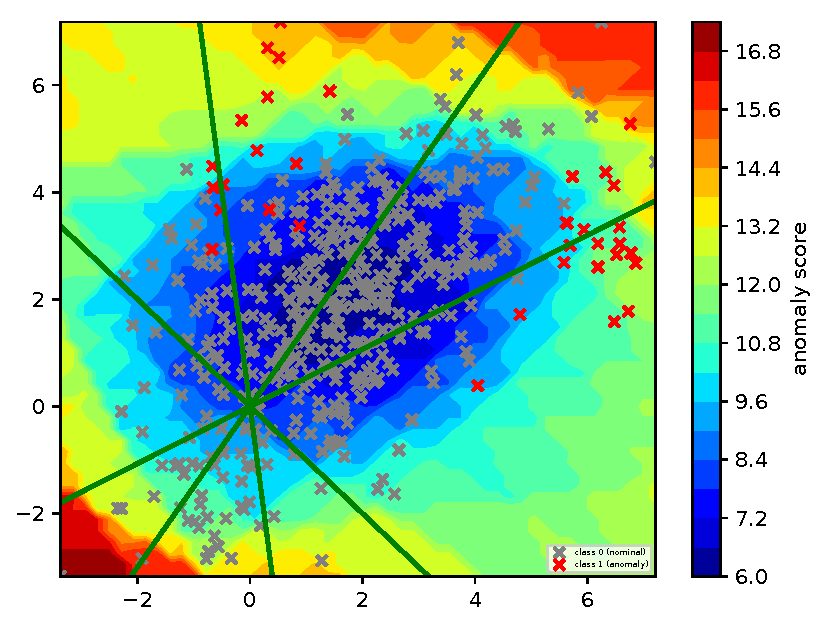
\includegraphics[width=0.48\textwidth]{figures/test_afss_toy2_loda_4w.pdf} \label{fig:loda_all}} 
	\subfloat[Score contours for each LODA projection]{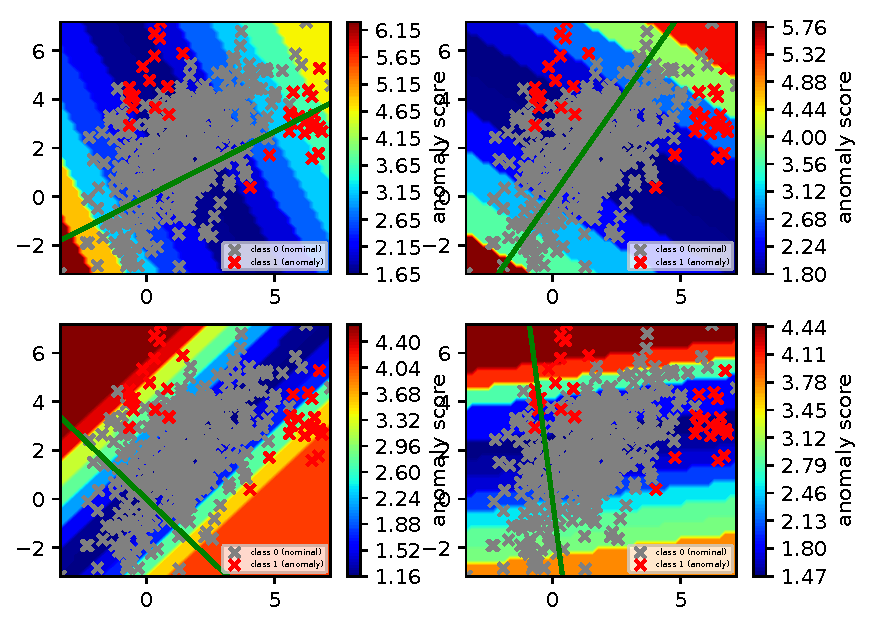
\includegraphics[width=0.48\textwidth]{figures/test_loda_toy2_active_4w_ensemble.pdf} \label{fig:loda_scores}} \\
	\subfloat[Initial uniform relevance ($b=0.5$)]{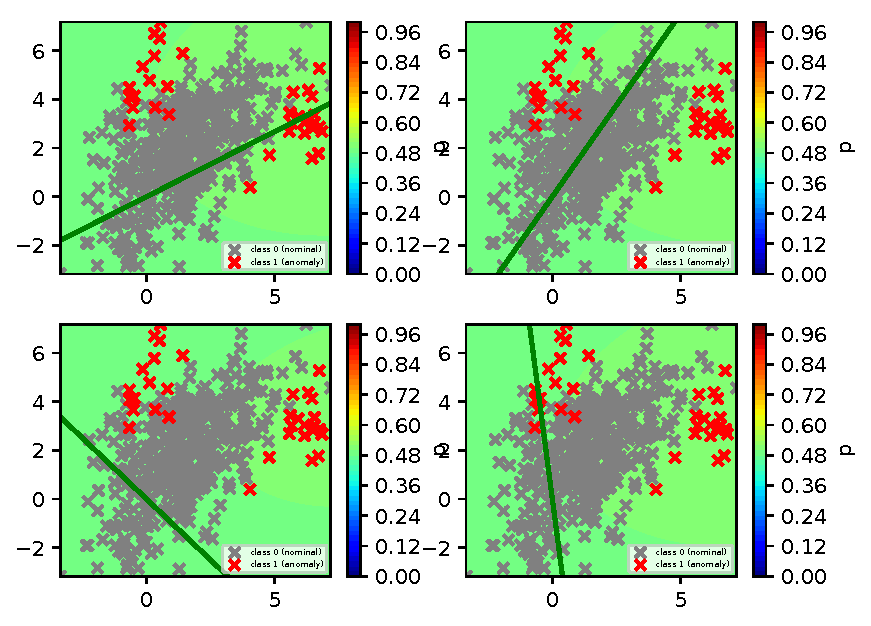
\includegraphics[width=0.48\textwidth]{figures/test_afss_toy2_active_4w_before.pdf} \label{fig:loda_uniform}} 
	\subfloat[Relevance after 30 feedback iterations]{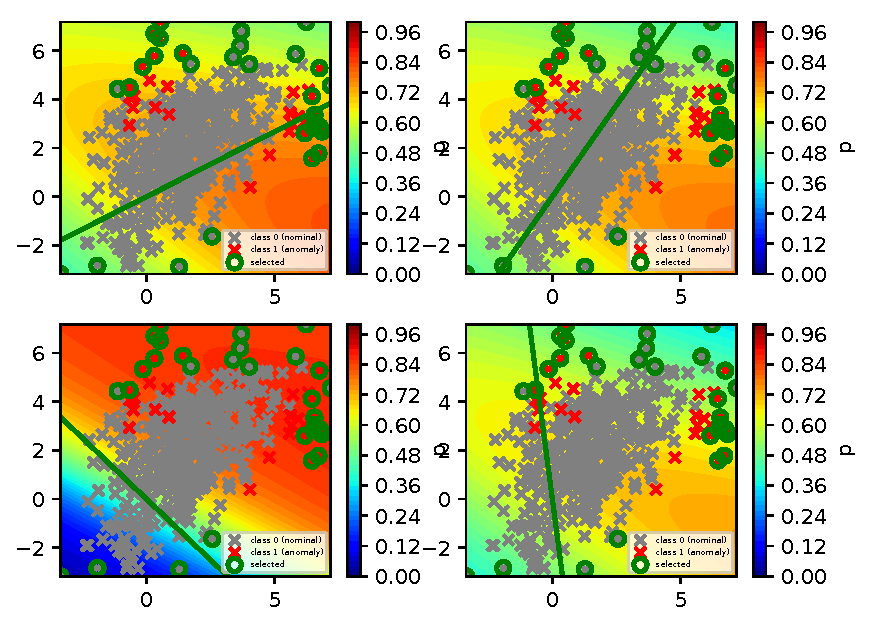
\includegraphics[width=0.48\textwidth]{figures/test_afss_toy2_active_4w_f30_after.pdf} \label{fig:loda_relevance}} \\[-1ex]
	\caption{\textit{Toy} data. More red on the \textbf{top row} indicates more \textit{anomalous}. More red on the \textbf{bottom row} indicates more \textit{relevant}. The red `$\times$' are true anomalies and grey `$\times$' are true nominals. {\bf (a)} LODA with four projections (green lines) applied to the \textit{Toy} dataset. {\bf (b)} The contours of only the \textit{bottom left} LODA projection are somewhat aligned with the true anomalies, i.e., most anomalies lie in the higher anomaly score regions. Other projections are highly inaccurate. {\bf (c)} The output nodes of the FSSN are initially primed to return a relevance of $0.5$ everywhere in the feature space. {\bf (d)} The points circled in green were shown to the analyst for labeling, one per feedback iteration. After $30$ iterations, the bottom left projection was found to be most relevant in the top-right half-space, whereas it is completely irrelevant in the bottom-left half-space. Other projections were less relevant in most parts of the feature space.}
	\label{fig:dataset}
\end{figure*}

\paragraph{Toy Data} The \textit{Toy} dataset and the corresponding LODA ensembles have been shown below as an illustration of how GLAD works. We find that GLAD learns useful relevance information that can be of help to the analyst.

\end{document}
